\chapter{Experiments}
\label{chap:Experiments}

\section{Dataset and Evaluation Metrics}
\label{sec:dataset_and_metrics}
To evaluate the proposed method, the Obama dataset from AD-NeRF~\cite{guo2021ad} was used, maintaining the same data split for training and testing.
Given the availability of ground truth for the same identity, metrics such as PSNR and LPIPS~\cite{zhang2018perceptual} can be utilized for Quantitative evaluation.

% on a single NVIDIA GeForce RTX 3090 GPU.

\section{Quantitative Evaluation Results. }
\label{sec:eval_Quantitative}
In Table \ref{tab:Quantitative}, a comparison of each model's PSNR, LPIPS, and real-time performance is presented, specifically when audio input is provided.
The MakeItTalk model~\cite{zhou2020makelttalk} is unable to replicate the exact head poses found in the ground truth video,
hence PSNR and LPIPS metrics are not reported for it.
Inference FPS data is collected in RTX 3090 GPU with Intel Zeon 6230R CPU environment.
\begin{table*}[t]
\begin{center}
\setlength{\tabcolsep}{10pt}
\renewcommand{\arraystretch}{1.1}
\begin{tabular}{l cc  ccc cc} 
\hline
Methods                              & PSNR[DB]$\uparrow$ & LPIPS$\downarrow$ & Training Time$\downarrow$ & Inference FPS$\uparrow$  \\   
Ground Truth                         & $\infty$       &  $0$              & -                         & -   \\
\hline
MakeItTalk~\cite{zhou2020makelttalk} & -       & -         & -     & $9$            \\
Wav2Lip~\cite{prajwal2020lip}        & $30.94$ & $0.0639$ & -     & $11$            \\
AD-NeRF~\cite{guo2021ad}             & $25.53$ & $0.0901$ & $36$h & $0.07$          \\
Rad-NeRF~\cite{tang2022radnerf}      & $34.00$ & $0.0387$ & $\mathbf{8}$h  & $\mathbf{51.64}$ \\
\hline
Ours                                 & $\mathbf{35.29}$ & $\mathbf{0.0360}$ & $\mathbf{8}$h  & $\mathbf{60.12}$ \\

\hline 
\end{tabular}
\end{center}
\vspace{-0.3cm}
\caption{\textbf{Quantitative comparison under real audio condition.} 
}
\label{tab:Quantitative}
\end{table*}

\section{Qualitative Evaluation Results. }
\label{sec:eval_Qualitative}
\begin{figure}
    \centering
    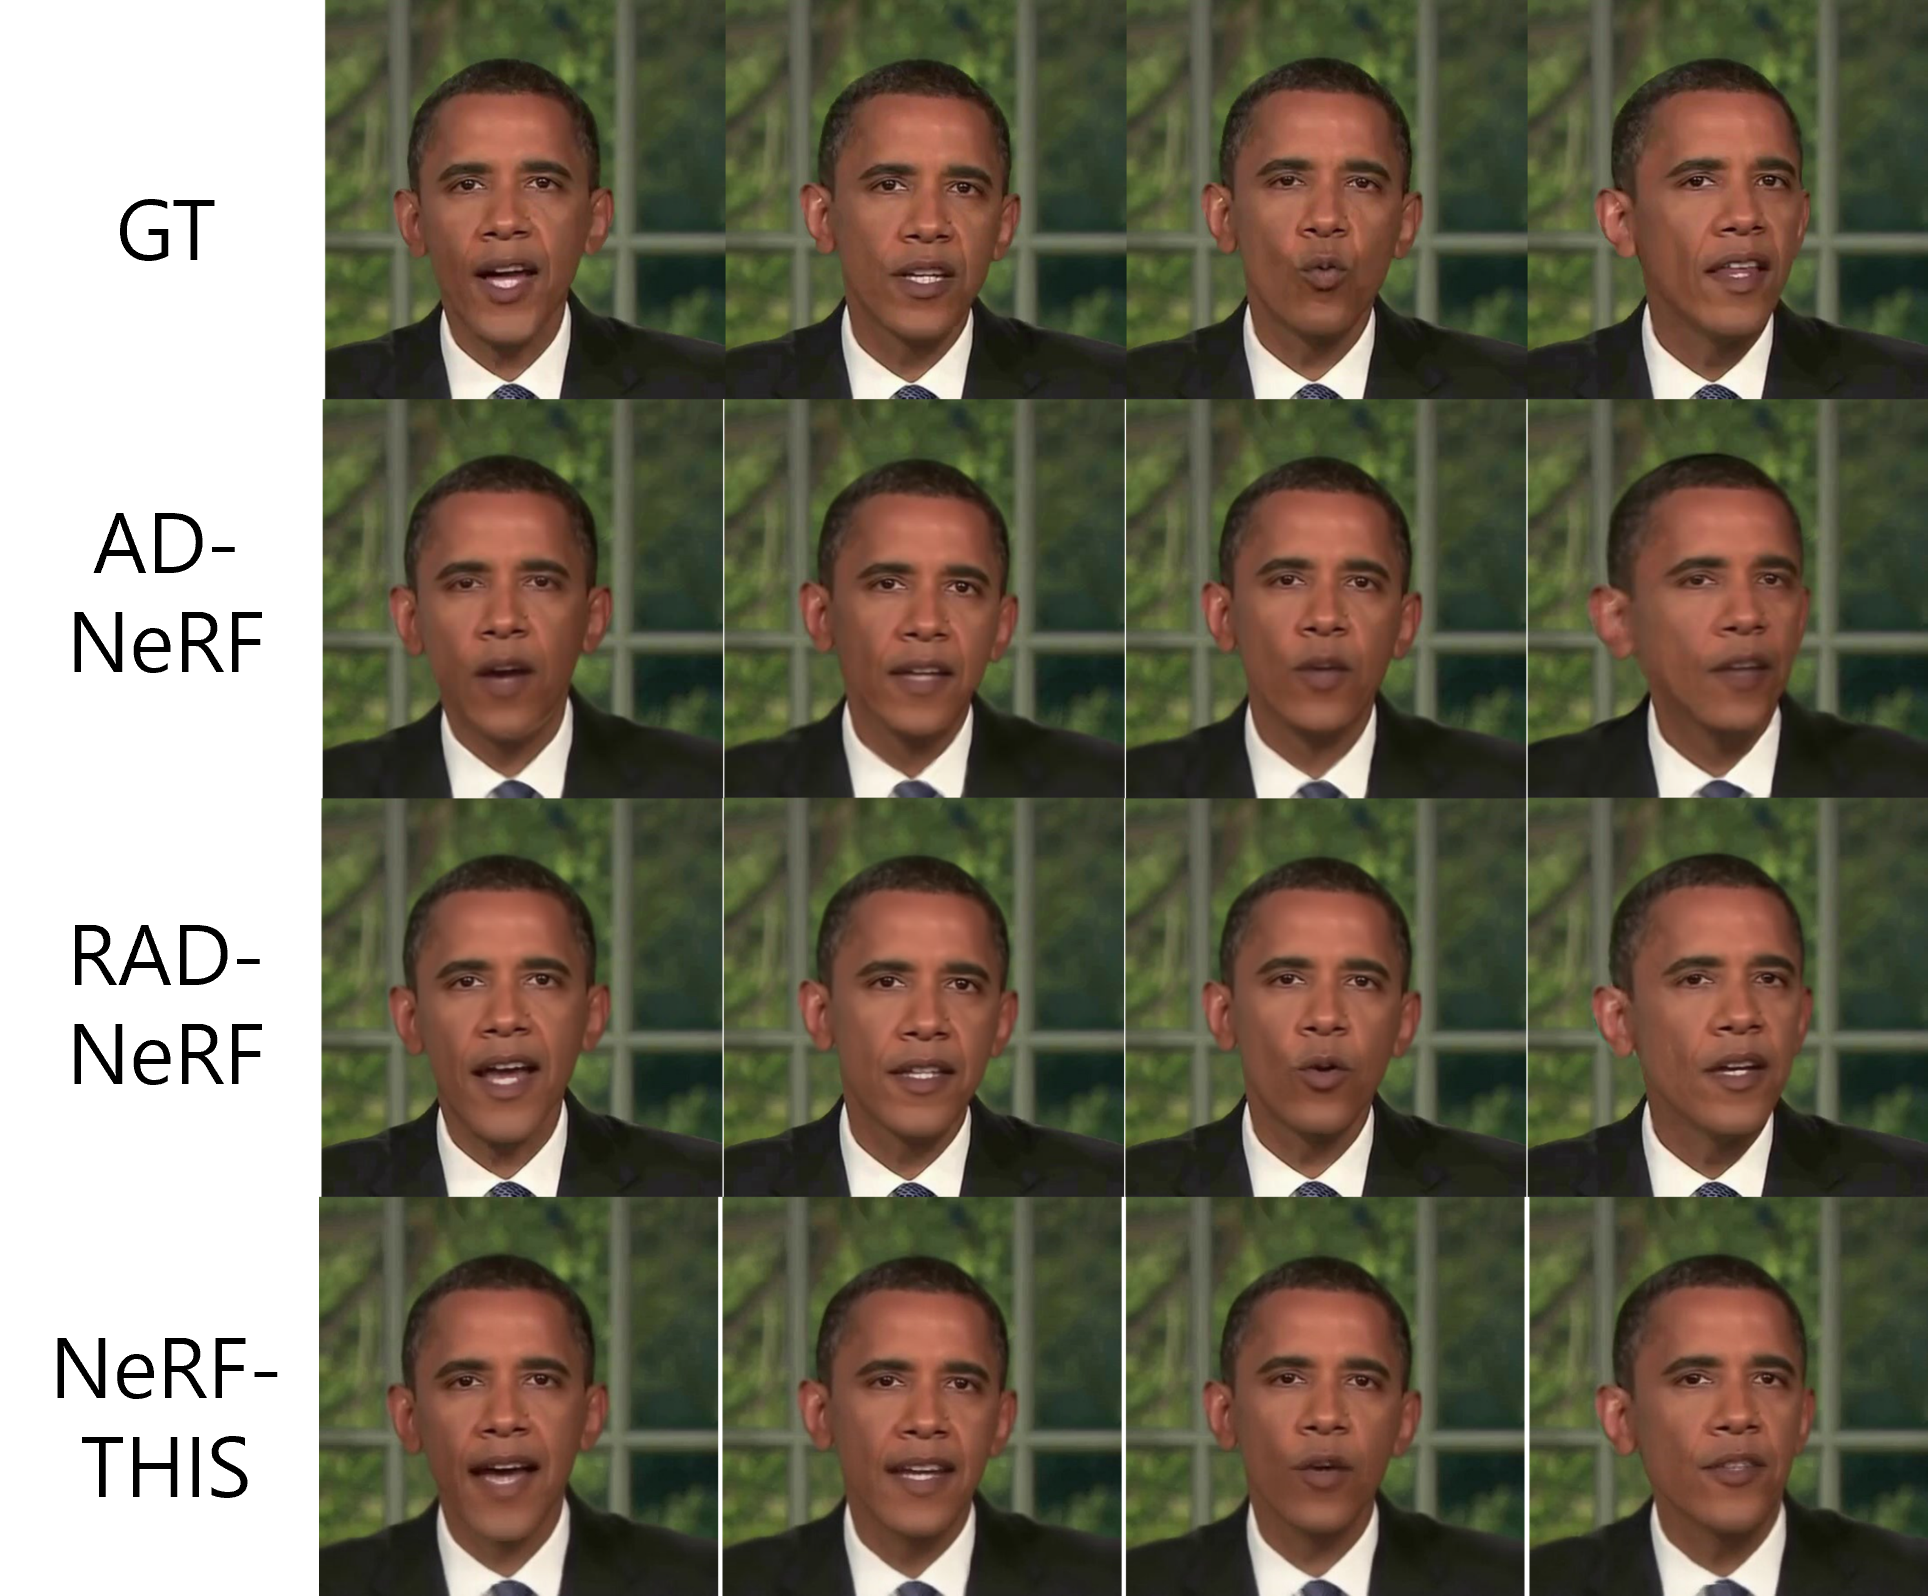
\includegraphics[width=0.8\textwidth]{figures/figure_chap_4/qualitative.png}
    \caption{Qualitative evaluation results}
    \label{fig:qualitative}
\end{figure}
\begin{table*}[t]
\begin{center}
\small
\renewcommand{\arraystretch}{1.1}
\begin{tabular}{l c c c c c c c c} 
\hline
Methods       & AD-NeRF~\cite{guo2021ad} & RAD-NeRF~\cite{tang2022radnerf} & Ours \\   
\hline
Audio-Lips Sync & 3.21 & 3.71 & 3.60 \\
Image Quality & 3.14 & 3.93 & 3.64\\
Boader Effacts & 2.53 & 3.69 & 3.79 \\
Image Transition & 2.72 & 3.70 & 3.84 \\
\hline 
\end{tabular}
\end{center}
\vspace{-0.3cm}
\caption{\textbf{User study.} 
The rating is of scale 1-5, the higher the better.
}
\label{tab:userstudy}
\end{table*}
\ref{fig:qualitative} represents, in order from top to bottom, GT (Ground Truth), AD-NeRF, Rad-NeRF, and the Proposed model.

The proposed model is designed to be trained with a smaller amount of input data.
As a result, while it may slightly lag behind other models in terms of textural details, it excels in accurately replicating eye movements and lip expressions.
This focus on nuanced facial movements, particularly in the eyes and mouth, enables the model to achieve superior performance in these areas, despite the trade-off in texture quality.

\subsection{User Study}
\label{sec:user_study}
To conduct a thorough assessment of the quality of generated talking faces, a comprehensive user study is organized with the participation of 10 attendees.
This study involves the evaluation of 10 synthesized videos, created through various methods in a cross-driven context.
The attendees focus on three key aspects: the synchronization of audio with lip movements, the quality of the image generation, and the overall realism of the videos.
This evaluation aims to determine the effectiveness and authenticity of different synthetic video generation techniques.
The results of this user study are shown in Table \ref{tab:userstudy}.
\begin{table*}[t]
\begin{center}
\small
\renewcommand{\arraystretch}{1.1}
\begin{tabular}{l c c c c c c c c} 
\hline
Methods       & AD-NeRF~\cite{guo2021ad} & RAD-NeRF~\cite{tang2022radnerf} & Ours \\   
\hline
Audio-Lips Sync & 3.21 & 3.71 & 3.60 \\
Image Quality & 3.14 & 3.93 & 3.64\\
Boader Effacts & 2.53 & 3.69 & 3.79 \\
Image Transition & 2.72 & 3.70 & 3.84 \\
\hline 
\end{tabular}
\end{center}
\vspace{-0.3cm}
\caption{\textbf{User study.} 
The rating is of scale 1-5, the higher the better.
}
\label{tab:userstudy}
\end{table*}
The proposed model outperforms in the boader effact perspective while the RAD-NeRF model~\cite{tang2022radnerf} is rated higher in terms of border effects.

\section{Advantages of TTS-integrated Synthesis}
In this context, the focus is on examining the advantages of simultaneously generating Text-to-Speech (TTS) along with the visual components,
compared to a cascading approach where the voice is generated separately and sequentially. 

\subsection{Synchronization}
\label{sec:synchronization}
When an avatar trained on Barack Obama's data was generated using a voice synthesized from the voice of a different author, it was observed that the sync quality with the original audio was compromised.
This discrepancy can be attributed to differences in voice characteristics such as volume and timbre between the synthesized voice and Obama's original voice. These domain differences highlight the challenges in achieving seamless audio-visual synchronization in avatars when the audio used for synthesis differs significantly from the data the avatar model was trained on.
However, it was found that utilizing tokens generated during the Text-to-Speech (TTS) process yielded better synchronization rates compared to the method of generating the talking head after the audio synthesis.
This suggests that integrating TTS-generated tokens directly into the talking head generation process allows for more accurate and synchronized movements of the facial features, particularly the lips, to match the speech. This approach indicates a more efficient and cohesive method for creating lifelike and synchronized talking avatars.
These performance improvements were confirmed in a user study\ref{tab:userstudy}, where it was found that using more compressed encoded tokens achieved similar performance to that of ASR (Automatic Speech Recognition) tokens.

\subsection{Efficiency}
\label{sec:efficiency}

When leveraging tokens generated during the Text-to-Speech (TTS) process for facial synthesis, a comparative analysis was conducted to evaluate how much more efficient this method is in terms of synthesis time, especially when compared to the cascading approach of synthesis. This comparison was made across varying lengths of audio, to understand the impact of audio duration on the synthesis efficiency. The aim was to determine if using TTS-generated tokens directly in facial synthesis significantly reduces the time required for the process, and how this efficiency scales with longer or shorter audio inputs.
This comperison is shown in Table \ref{tab:efficiency}, where the models to inference were aleady loaded onto the GPU.
While there is a clear difference in efficiency between using TTS-generated tokens for facial synthesis and the cascading approach, it was observed that external factors, such as the time taken to complete the video processing with ffmpeg, significantly impact the overall performance. This means that the improvements gained from the model's efficiency in facial synthesis were somewhat offset by the time required for video completion through ffmpeg. As a result, the expected level of efficiency improvement was not fully realized due to these external processing factors. 
\begin{table}
    \centering
    \begin{tabular}{ccc}
        \hline
        Audio Duration & End-to-End & Cascading \\
        \hline
        7s & 4.41s & 6.83s \\
        \hline
        15s & 12.87s & 16.24s \\
        \hline
    \end{tabular}
    \caption{Comparison of synthesis time for TTS-integrated and cascading approaches}
    \label{tab:efficiency}
\end{table}